\documentclass[a4paper,12pt]{extarticle}
\usepackage[utf8x]{inputenc}
\usepackage[T1,T2A]{fontenc}
\usepackage[russian]{babel}
\usepackage{hyperref}
\usepackage{indentfirst}
\usepackage{listings}
\usepackage{color}
\usepackage{here}
\usepackage{array}
\usepackage{multirow}
\usepackage{graphicx}
\usepackage{amsmath}
\usepackage{amssymb}
\usepackage{makeidx}    

\usepackage{caption}
\renewcommand{\lstlistingname}{Программа} % заголовок листингов кода

\bibliographystyle{ugost2008ls}

\usepackage{listings}
\lstset{ %
extendedchars=\true,
keepspaces=true,
language=C,						% choose the language of the code
basicstyle=\footnotesize,		% the size of the fonts that are used for the code
numbers=left,					% where to put the line-numbers
numberstyle=\footnotesize,		% the size of the fonts that are used for the line-numbers
stepnumber=1,					% the step between two line-numbers. If it is 1 each line will be numbered
numbersep=5pt,					% how far the line-numbers are from the code
backgroundcolor=\color{white},	% choose the background color. You must add \usepackage{color}
showspaces=false				% show spaces adding particular underscores
showstringspaces=false,			% underline spaces within strings
showtabs=false,					% show tabs within strings adding particular underscores
frame=single,           		% adds a frame around the code
tabsize=2,						% sets default tabsize to 2 spaces
captionpos=t,					% sets the caption-position to top
breaklines=true,				% sets automatic line breaking
breakatwhitespace=false,		% sets if automatic breaks should only happen at whitespace
escapeinside={\%*}{*)},			% if you want to add a comment within your code
postbreak=\raisebox{0ex}[0ex][0ex]{\ensuremath{\color{red}\hookrightarrow\space}},
texcl=true,
inputpath=source,                     % директория с листингами
}

\usepackage[left=2cm,right=2cm,
top=2cm,bottom=2cm,bindingoffset=0cm]{geometry}

%% Нумерация картинок по секциям
\usepackage{chngcntr}
\counterwithin{figure}{section}
\counterwithin{table}{section}

%%Точки нумерации заголовков
\usepackage{titlesec}
\titlelabel{\thetitle.\quad}
\usepackage[dotinlabels]{titletoc}

%% Оформления подписи рисунка
\addto\captionsrussian{\renewcommand{\figurename}{Рисунок}}
\captionsetup[figure]{labelsep = period}

%% Подпись таблицы
\DeclareCaptionFormat{hfillstart}{\hfill#1#2#3\par}
\captionsetup[table]{format=hfillstart,labelsep=newline,justification=centering,skip=-10pt,textfont=bf}

%% Путь к каталогу с рисунками
\graphicspath{{pictures/}}


\begin{document}	% начало документа

% Титульная страница
\begin{titlepage}	% начало титульной страницы

	\begin{center}		% выравнивание по центру

		\large Санкт-Петербургский Политехнический Университет Петра Великого\\
		\large Институт компьютерных наук и технологий \\
		\large Кафедра компьютерных систем и программных технологий\\[6cm]
		% название института, затем отступ 6см
		
		\huge Телекоммуникационные технологии\\[0.5cm] % название работы, затем отступ 				%0,5см
		\large Отчет по лабораторной работе №3\\[0.1cm]
		\large Линейная фильтрация
		\\[5cm]

	\end{center}


	\begin{flushright} % выравнивание по правому краю
		\begin{minipage}{0.25\textwidth} % врезка в половину ширины текста
			\begin{flushleft} % выровнять её содержимое по левому краю

				\large\textbf{Работу выполнил:}\\
				\large Балсутьев В.А.\\
				\large {Группа:} 33501/4\\
				
				\large \textbf{Преподаватель:}\\
				\large Богач Н.В.

			\end{flushleft}
		\end{minipage}
	\end{flushright}
	
	\vfill % заполнить всё доступное ниже пространство

	\begin{center}
	\large Санкт-Петербург\\
	\large \the\year % вывести дату
	\end{center} % закончить выравнивание по центру

\thispagestyle{empty} % не нумеровать страницу
\end{titlepage} % конец титульной страницы

\vfill % заполнить всё доступное ниже пространство
	

% Содержание
% Содержание
\renewcommand\contentsname{\centerline{Содержание}}
\tableofcontents
\newpage




\section{Цель работы}
Изучение методов модуляции цифровых сигналов.

\section{Теоретическая информация}

В настоящее время все большая часть информации, передаваемой по разнообразным каналам связи, существует в цифровом виде. Это означает, что передаче подлежит не непрерывный (аналоговый) модулирующий сигнал, а последовательность целых чисел по $ n_0, n_1,  n_2, ... $, которые могут принимать значения из некоторого фиксированного конечного множества. Эти числа, называемые символами (symbol), поступают от источника информации с периодом $ T $, а частота, соответствующая этому периоду, называется символьной скоростью (symbol rate): $ f_T =  1/T $.

Последовательность передаваемых символов является, очевидно, дискретным сигналом. Поскольку символы принимают значения из конечного множества, этот сигнал фактически является и квантованным, то есть цифровым сигналом. 
Типичный подход при осуществлении передачи дискретной последовательности символов состоит в следующем. Каждому из возможных значений символа сопоставляется некоторый набор параметров несущего колебания. Эти параметры поддерживаются постоянными в течение интервала $ T $, то есть до прихода следующего символа. Фактически это означает преобразование последовательности чисел (${n_k}$) в ступенчатый сигнал $ S_n(t) $ с использованием кусочно-постоянной интерполяции:

$$s_n(t) = f(n_k), kT < t < (k + 1)T$$. 

Здесь $f$ — некоторая функция преобразования. Полученный сигнал $s_n(t)$ далее используется в качестве модулирующего сигнала обычным способом.
Такой способ модуляции, когда параметры несущего колебания меняются скачкообразно, называется манипуляцией (keying). В зависимости от того, какие именно параметры изменяются, различают амплитудную (АМн), фазовую (ФМн), частотную (ЧМн) и квадратурную (КАМн) манипуляцию. Кроме того, при передаче цифровой информации может использоваться несущее колебание, отличное по форме от гармонического. Так, при использовании в качестве несущего колебания последовательности прямоугольных импульсов возможны амплитудно-импульсная (АИМ), широтно-импульсная (ШИМ) и время-импульсная (ВИМ) модуляция.

\subsection{Частотная манипуляция}
При частотной манипуляции (ЧMн; английский термин — frequency shift keying, FSK) каждому возможному значению передаваемого символа сопоставляется своя частота. В течение каждого символьного интервала передается гармоническое колебание с частотой, соответствующей текущему символу.

\subsection{Минимальная частотная манипуляция}
Для повышения помехоустойчивости ЧМн желательно, чтобы посылки, соответствующие разным символам, были некоррелированы. Считая начальные фазы посылок нулевыми, ЧМн-сигналы для символов 0 и 1 можно записать так: 
$$ s_0(t) = A \cos(\omega_0 t), 0 <= t <= T $$
$$ s_1(t) = A \cos(\omega_1 t), 0 <= t <= T $$
Их ВКФ при нулевом временном сдвиге равна
$$ B_{01} = \int_{0}^{T} s_0(t)s_1(t)dt = A^2 \int_{0}^{T} \cos( \omega_0 t ) \cos( \omega_1 t)dt =
\frac{A^2 \sin(\omega_1 + \omega_1)T}{2(\omega_1 + \omega_0)} + \frac{A^2 \sin(\omega_1 - \omega_0)T}{2(\omega_1 - \omega_0)}. $$
 
Если $ (\omega_1 + \omega_0)T >> 1 $, то первое слагаемое значительно меньше второго и им можно пренебречь:
$$ B_{01} = \frac{A^2 \sin(\omega_1 - \omega_0) T}{2(\omega_1 - \omega_0)} $$
Это значени равно нулю при $ (\omega_1 - \omega_0)T = \pi k, $ где $k$ - целое число, не равное нулю.
Таким образом, минимальное значение расстояния междк частотами манипуляции, при котором посылки, соответствующие разным символам, оказываются некоррелированными, составляет:

$$ \delta \omega_{min} = \frac{\pi}{T}, \delta f_{min} = \frac{1}{2T} = \frac{f_T}{2}, $$

где $ f_T $ - символьная скорость.

Двухпозиционная(бинарная) ЧМн, частоты которой выбраны согласно последней формуле, получила
название минимальной частотной манипуляции(minimal shift keying MSK).  


\subsection{Фазовая манипуляция}

Фазовая манипуляция (phase-shift keying PSK) — один из видов фазовой модуляции, при которой фаза несущего колебания меняется скачкообразно в зависимости от информационного сообщения.

Фазоманипулированный сигнал имеет следующий вид:
$$ s_m(t) = g(t) \cos(2 \pi f_ct + \phi_m(t)), $$
где $g(t)$ определяет огибающую сигнала; $\phi_m(t)$ является модулирующим сигналом. $\phi_m(t)$  может принимать  $M$ дискретных значений. $f_c$  — частота несущей.

\subsubsection{Двоичная фазовая манипуляция}
Двоичная фазовая манипуляция (binary phase-shift keying BPSK) — самая простая форма фазовой манипуляции. Работа схемы двоичной ФМн заключается в смещении фазы несущего колебания на одно из двух значений, нуль или $\pi$(180°). Двоичную фазовую манипуляцию можно также рассматривать как частный случай квадратурной манипуляции (QAM-2).

\subsubsection{Квадратурная фазовая манипуляция}
При квадратурной фазовой манипуляции (Quadrature Phase Shift Keying QPSK или 4-PSK) используется созвездие из четырёх точек, размещённых на равных расстояниях на окружности. Используя 4 фазы, в QPSK на символ приходится два бита, как показано на рисунке. Анализ показывает, что скорость может быть увеличена в два раза относительно BPSK при той же полосе сигнала, либо оставить скорость прежней, но уменьшить полосу вдвое.
Хотя QPSK можно считать квадратурной манипуляцией (QAM-4), иногда её проще рассматривать в виде двух независимых модулированных несущих, сдвинутых на 90°. При таком подходе чётные (нечётные) биты используются для модуляции синфазной составляющей 	$I$, а нечётные (чётные) — квадратурной составляющей несущей $Q$. Так как BPSK используется для обеих составляющих несущей, то они могут быть демодулированы независимо.

\subsubsection{Квадратурная фазовая манипуляция}
При квадратурной фазовой модуляции наблюдается непостоянство огибающей сигнала. Уменьшить изменения огибающей сигнала с квадратурной фазовой модуляцией, вызванные ограничением полосы, можно введением задержки модулирующего сигнала в квадратурном канале по отношению к синфазному каналу. Этот вид модуляции назвается квадратурной фазовой манипуляцией со сдвигом (offset quadrature phase shift keying OQPSK). При такой модуляции квадратурные составляющие модулирующего сигнала смещены во времени на величину половины длительности символа. Благодаря этому исключаются изменения фазы.


\section{Ход выполнения работы}
\subsection{BPSK}
Вспользовавшись стадартными функциями MATLAB и пакета Signal Proccesing, получаем созвездие 
двоичной фазовой манипуляции.

\begin{figure}[H]
	\begin{center}
		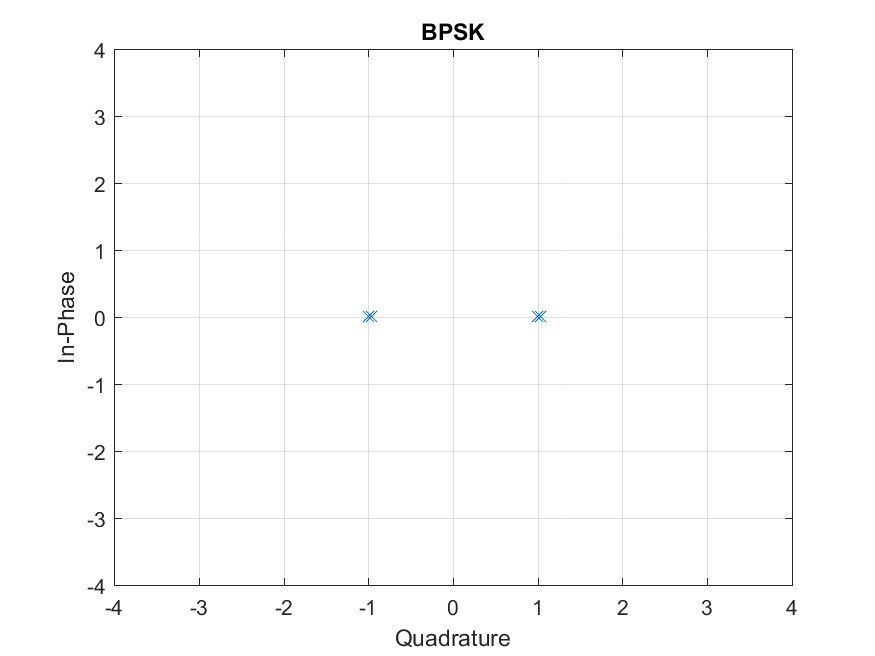
\includegraphics[scale=0.7]{bpsk.png}
		\caption{BPSK} 
		\label{pic:bpsk} % название для ссылок внутри кода
	\end{center}
\end{figure} 

\subsection{PSK}
Далее действуя аналогичным образом, построим созвездие для общего случая фазовой манипуляции. 

\begin{figure}[H]
	\begin{center}
		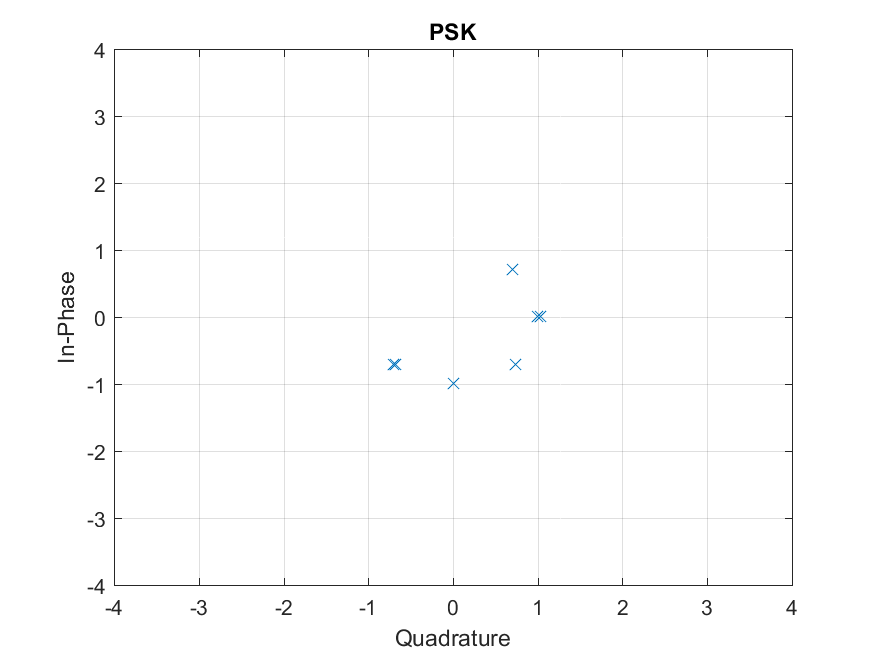
\includegraphics[scale=0.7]{psk.png}
		\caption{PSK} 
		\label{pic:psk} % название для ссылок внутри кода
	\end{center}
\end{figure} 

\subsection{OQPSK}

Теперь построим созвездие при квадратурной манипуляции со сдвигом.
\begin{figure}[H]
	\begin{center}
		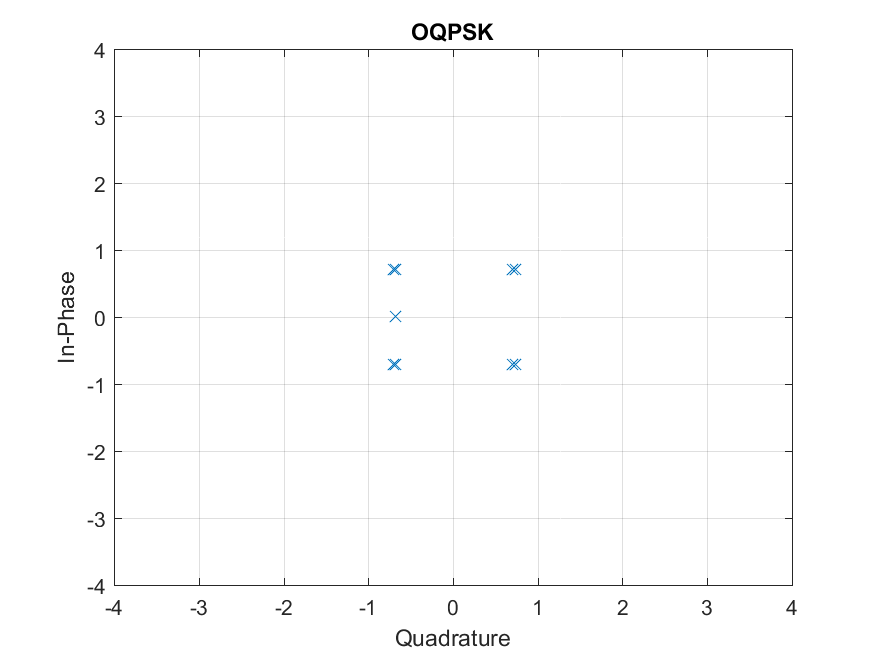
\includegraphics[scale=0.7]{oqpsk.png}
		\caption{OQPSK} 
		\label{pic:oqpsk} % название для ссылок внутри кода
	\end{center}
\end{figure} 

\subsection{genQAM}
Далее рассмотрим обычную квадратурной модуляции и его созвездие.
\begin{figure}[H]
	\begin{center}
		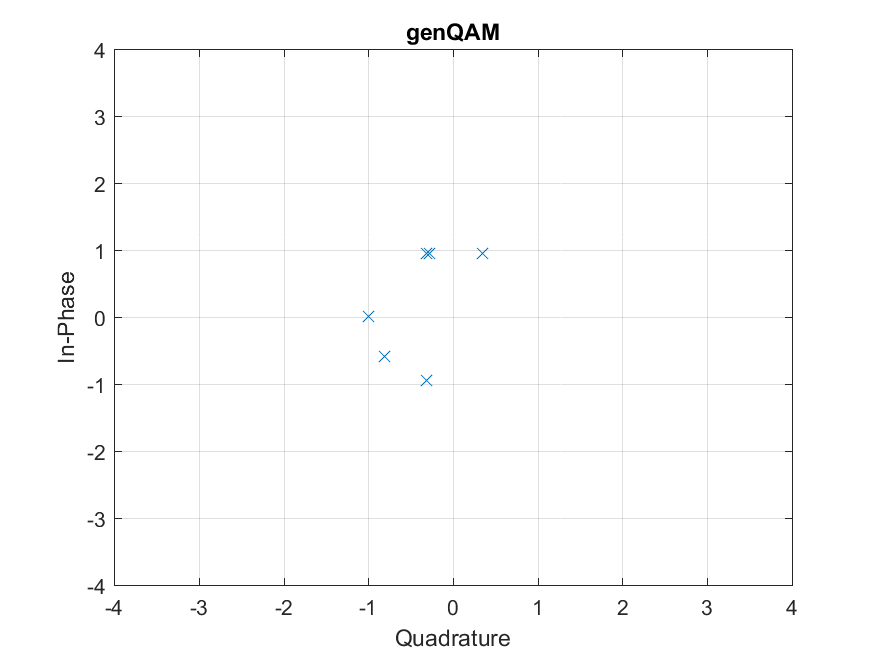
\includegraphics[scale=0.7]{genqam.png}
		\caption{genQAM} 
		\label{pic:genqam} % название для ссылок внутри кода
	\end{center}
\end{figure} 

\subsection{MSK}

Теперь построим созвездие минимальной частотной модуляции. 
\begin{figure}[H]
	\begin{center}
		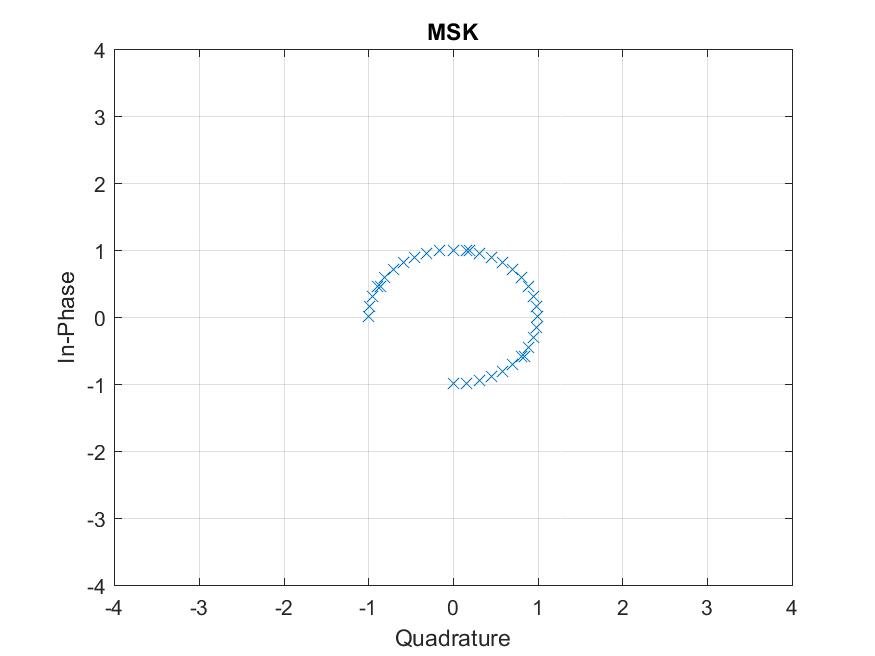
\includegraphics[scale=0.7]{msk.png}
		\caption{MSK} 
		\label{pic:msk} % название для ссылок внутри кода
	\end{center}
\end{figure} 


\lstinputlisting[
	label=code:source01,
	caption={lab06.m},% для печати символ '_' требует выходной символ '\'
]{lab06.m}
\parindent=1cm % командна \lstinputlisting сбивает параментры отступа


\subsection{Выводы}
\noindent Цифровая модуляция — процесс преобразования последовательности кодовых символов в последовательность элементов сигнала. Существуют следующие типы манипуляций: частотная манипуляция, фазовая манипуляция, амплитудная манипуляция, квадратурная амплитудная манипуляция.\\
Квадратурная амплитудная манипуляция(QAM) — манипуляция, при которой изменяется как фаза, так и амплитуда сигнала, что позволяет увеличить количество информации, передаваемой одним состоянием сигнала. \\
Фазовая манипуляция(PSK) — один из видов фазовой модуляции, при которой фаза несущего колебания меняется скачкообразно в зависимости от информационного сообщения.\\
Двоичная фазовая манипуляция — самая простая форма фазовой манипуляции. Работа схемы двоичной ФМн заключается в смещении фазы несущего колебания на одно из двух значений, нуль или $\pi (180\circ)$. Двоичную фазовую манипуляцию можно также рассматривать как частный случай квадратурной манипуляции (QAM-2).\\
При квадратурной фазовой манипуляции(QPSK) используется созвездие из четырёх точек, размещённых на равных расстояниях на окружности. Используя 4 фазы, в QPSK на символ приходится два бита. Анализ показывает, что скорость может быть увеличена в два раза относительно BPSK при той же полосе сигнала, либо оставить скорость прежней, но уменьшить полосу вдвое.\\
Частотная манипуляция с минимальным сдвигом(MSK) представляет собой способ модуляции, при котором не происходит скачков фазы и изменение частоты происходит в моменты пересечения несущей нулевого уровня. MSK уникальна потому, что значение частот соответствующих логическим «0» и «1» отличаются на величину равную половине скорости передачи данных. Другими словами, индекс модуляции равен 0,5.\\
Уровень модуляции определяет количество состояний несущей, используемых для передачи информации. Чем выше этот уровень, тем большими скоростными возможностями и меньшей помехоустойчивостью модуляция обладает. Число бит, передаваемых одним состоянием, определяется как $Log N$, где N — уровень модуляции. Таким образом, чем выше уровень модуляции, тем больше данных мы можем передать (или потерять) за единицу времени.
\end{document}
